\documentclass[11pt, english, fleqn, DIV=15, headinclude, BCOR=2cm]{scrreprt}

\usepackage[
    color,
    bibatend,
]{../../header}

\graphicspath{{./}{../Figures/}}

\newcommand\MZ{M_{\mathrm Z^0}}
\newcommand\electron{\mathrm e^-}
\newcommand\positron{\mathrm e^+}

\usepackage{mathtools}

\hypersetup{
    pdftitle=
}

\usepackage{longtable}
\usepackage{subcaption}

\usepackage[all]{nowidow}

\newcommand\ecal{\emph{e-cal}}
\newcommand\hcal{\emph{h-cal}}
\newcommand\sump{\emph{sum-p}}

\subject{Lab report}
\title{Analysis of $Z_0$ decays}
\subtitle{Experiment E213 -- Universität Bonn}
\author{%
    Martin Ueding \\
    \small{\href{mailto:mu@martin-ueding.de}{mu@martin-ueding.de}}
    \and
    Lino Lemmer \\
    \small{\href{mailto:l2@uni-bonn.de}{l2@uni-bonn.de}}
}

\date{2016-03-02}

\publishers{Tutor: David Hohn}

\begin{document}

\maketitle

\begin{abstract}
    In this experiment we analyse data from electron positron collisions
    collected with the \textsc{opal} detector at the \textsc{lep} collider.
    Aim of the experiment is to have an insight in methods of data analysis in
    high energy physics.
    
    In the first part we learn to distinguish between the different decay
    channels of the $\mathrm{Z}^0$ boson by their signature in the detector
    with a small data sample.

    In the second part we want to find mass, decay width and partial cross
    section of the $\mathrm{Z}^0$ for different decay channels and the weak
    mixing angle angle from the forward backward asymmetry of the
    $\electron\positron \to \muup^-\muup^+$ reaction. We also want to verify
    the lepton universality and to identify the number of neutrino generations.
    For this part we use preselected data and Monte Carlo events as help.
\end{abstract}

\tableofcontents

\chapter*{Permission to upload}

I, Martin Ueding, would like to scan and upload this lab report with your
corrections to my website \href{http://martin-ueding.de}{martin-ueding.de}.
There, the original lab report as well as the reviewed one will be licensed
under the “\href{http://creativecommons.org/licenses/by-sa/4.0/}{Creative
Commons Attribution-ShareAlike 4.0 International License}”. Is that okay with
you?

Yes $\Box$ \hspace{2cm} No $\Box$

\chapter{Theory}

\section{The OPAL detector}

% TODO Delete the following line.
Y'know, there are those calorimeters. It ain't 'bout food 'n stuff.

Since \enquote{electromagnetic calorimeter} and \enquote{hadronic calorimeter}
is quite a mouthful, we will call them \ecal{} and \hcal{} from now on.

\section{Decay channels of the $\mathrm Z^0$ boson}

\subsection{Leptonic decay}

\subsection{Hadronic decay}

\section{Analysis methods}

\subsection{GROPE}

\subsection{Slice optimizing with Monte Carlo simulation}

\begin{figure}
    \centering
    \includegraphics{radiative_interpolation}
    \caption{%
        Radiation corrections given in the experiment description on page~4. We
        have interpolated with quadratic splines.
    }
    \label{fig:radiative_interpolation}
\end{figure}

\chapter{Exercises}

There are a couple of exercises that are supposed to be done before the
experiment.

\section{Decay width}

We are to compute the decay width~$\Gamma$ of a $\mathrm Z^0$ particle into a
pair of various fermions. The top-quark is heavier than the gauge boson,
therefore it cannot decay into a pair of top-quarks. The Feynman diagram
corresponding to the decay is shown in Figure~\ref{fig:z0-decay}.

\begin{figure}
    \centering
    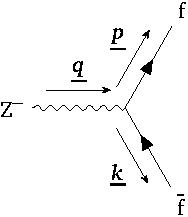
\includegraphics{z0-decay}
    \caption{%
        Decay of a $\mathrm Z^0$ gauge boson into a pair of fermions. Time is
        to the right.
    }
    \label{fig:z0-decay}
\end{figure}

First we compute the invariant matrix element~$\mathcal M$. Reading off the
Feynman diagram, we have
\begin{align*}
    \iup \mathcal M
    &= \epsilon^\mu \bar u^s(\four p) \frac{\iup g}{\cos(\theta_\text w)}
    \mat\gamma_\mu \del{g_\text v^f - g_\text a^f \mat\gamma_5} v^{s'}(\four k)
    \,,
    \intertext{%
        where we have used the rules given by \textcite[(D.56)]{romao/aqt}. We
        chose the center of mass system, as we always can for a single massive
        particle, and have $\four q = (\sqrt s, \vec 0)$. As the gauge boson
        does not have any three momentum direction, we can choose the
        polarization vector $\four \epsilon$ like we want. We chose it in the
        positive $x^3$-direction and have $\four \epsilon = (0, 0, 0, 1)$. With
        that we can simplify the Lorentz structure a little bit and obtain
    }
    &= \bar u^s(\four p) \frac{\iup g}{\cos(\theta_\text w)}
    \mat\gamma_3 \del{g_\text v^f - g_\text a^f \mat\gamma_5} v^{s'}(\four k)
    \,.
\end{align*}

For the decay width, which we are interested in, we need the modulus squared of
the matrix element. For that we need the following:
\begin{multline*}
    \sbr{\bar u^s(\four p) \mat\gamma_3 \del{g_\text v^f - g_\text a^f \mat\gamma_5}
    v^{s'}(\four k)}^\dagger \\
    =
    v^{s'}(\four k)^\dagger
    \del{g_\text v^f - g_\text a^f \mat\gamma_5^\dagger}
    \mat\gamma_3^\dagger
    \mat\gamma_0
    u^s(\four p) \\
    =
    \underbracket{v^{s'}(\four k)^\dagger
    \mat\gamma_0}
    \underbracket{\mat\gamma_0
        \del{g_\text v^f - g_\text a^f \mat\gamma_5^\dagger}
    \mat\gamma_0}
    \underbracket{\mat\gamma_0
        \mat\gamma_3^\dagger
    \mat\gamma_0}
    u^s(\four p) \\
    = \bar v^{s'}(\four k)
    \del{g_\text v^f + g_\text a^f \mat\gamma_5}
    \mat\gamma_3
    u^s(\four p) \\
    = \bar v^{s'}(\four k)
    \mat\gamma_3
    \del{g_\text v^f - g_\text a^f \mat\gamma_5}
    u^s(\four p) \,. \\
\end{multline*}

Now we can write the modulus squared of the matrix element
\begin{align*}
    |\mathcal M|^2
    &= \frac{g^2}{\cos(\theta_\text w)^2}
    \bar v^{s'}(\four k)
    \mat\gamma_3
    \del{g_\text v^f - g_\text a^f \mat\gamma_5}
    u^s(\four p)
    \bar u^s(\four p)
    \mat\gamma_3
    \del{g_\text v^f - g_\text a^f \mat\gamma_5}
    v^{s'}(\four k)
    \,. \\
    \intertext{%
        As the detector is not sensitive to the spin of the resulting fermions,
        we need to sum over all the final state spin configurations $s$ and
        $s'$. This will give us a fermion trace,
    }
    \sum_\text{spins} |\mathcal M|^2
    &=
    \frac{g^2}{\cos(\theta_\text w)^2}
    \tr\del{
        \four k
        \mat\gamma_3
        \del{g_\text v^f - g_\text a^f \mat\gamma_5}
        \four p
        \mat\gamma_3
        \del{g_\text v^f - g_\text a^f \mat\gamma_5}
    }
    \,, \\
    \intertext{%
        where we have neglected the masses of the fermions. The second
        parentheses with $\mat\gamma_5$ can be anticommuted twice and be
        collapsed with the first one. We have
    }
    &=
    \frac{g^2}{\cos(\theta_\text w)^2}
    \tr\del{
        \four k
        \mat\gamma_3
        \del{g_\text v^f - g_\text a^f \mat\gamma_5}^2
        \four p
        \mat\gamma_3
    }
    \,, \\
    \intertext{%
        where we can now simplify this. As an aside, we have
        \[
            \del{g_\text v^f - g_\text a^f \mat\gamma_5}^2
            = (g_\text v^f)^2 - (g_\text a^f)^2 - 2 g_\text v^f g_\text a^f
            \mat\gamma_5 \,.
        \]
        The square of $\mat\gamma_5$ is just the unit matrix in Dirac space.
        The term with $\mat\gamma_5$ will drop out as the trace identity
        contains the Levi-Civita symbol~$\epsilon_{\mu\nu\rho\gamma}$ which
        will be zero if two of the indices are 3, as we have in our case.
        Therefore we can directly drop that term. As it does not contain any
        further Dirac structure, we can pull it out front and obtain
    }
    &=
    \frac{g^2}{\cos(\theta_\text w)^2}
    \del{(g_\text v^f)^2 - (g_\text a^f)^2}
    \tr\del{
        \four k
        \mat\gamma_3
        \four p
        \mat\gamma_3
    }
    \,.
    \intertext{%
        Using a trace identity like given by \textcite[(A.27)]{Peskin/QFT/1995}
        we obtain
    }
    &= \frac{4 g^2}{\cos(\theta_\text w)^2} \del{(g_\text v^f)^2 - (g_\text a^f)^2}
    (2 k_3 p_3 + \four k \cdot \four p) \,.
\end{align*}
This is our final form of the matrix element.

The decay width is given by additional factors and a integration over phase
space. We have
\begin{align*}
    \Gamma_f
    &= \frac{1}{2 M_{\mathrm Z^0}} (2 \piup)^4 \int
    \frac{\dif^3 p}{(2\piup)^3 2 E_{\vec p}}
    \frac{\dif^3 k}{(2\piup)^3 2 E_{\vec k}}
    \delta^4(\four q - \four k - \four p)
    |\mathcal M|^2 \,.
    \intertext{%
        We simplify the factors and insert the matrix element and get
    }
    &= \frac{1}{32 \piup^2 M_{\mathrm Z^0}} \int
    \frac{\dif^3 p}{E_{\vec p}}
    \frac{\dif^3 k}{E_{\vec k}}
    \delta^4(\four q - \four k - \four p)
    \frac{4 g^2}{\cos(\theta_\text w)^2}
    \del{(g_\text v^f)^2 - (g_\text a^f)^2}
    (2 k_3 p_3 + \four k \cdot \four p) \,.
    \intertext{%
        Then we simplify even more and obtain
    }
    &= \frac{1}{8 \piup^2 M_{\mathrm Z^0}}
    \frac{g^2}{\cos(\theta_\text w)^2}
    \del{(g_\text v^f)^2 - (g_\text a^f)^2}
    \int
    \frac{\dif^3 p}{E_{\vec p}}
    \frac{\dif^3 k}{E_{\vec k}}
    \delta^4(\four q - \four k - \four p)
    (2 k_3 p_3 + \four k \cdot \four p) \,.
    \intertext{%
        The total energy-momentum conserving Dirac-distribution can be split
        into time-like and space-like part. In the center-of-mass frame, this
        gives us
    }
    &= \frac{1}{8 \piup^2 M_{\mathrm Z^0}}
    \frac{g^2}{\cos(\theta_\text w)^2}
    \del{(g_\text v^f)^2 - (g_\text a^f)^2}
    \\&\qquad\times
    \int
    \frac{\dif^3 p}{E_{\vec p}}
    \frac{\dif^3 k}{E_{\vec k}}
    \delta(\sqrt s - E_{\four k} - E_{\four p})
    \delta^3(\vec k + \vec p)
    (2 k_3 p_3 + \four k \cdot \four p) \,,
    \intertext{%
        which suggests the following change in variables:
        \[
            \vec a := \vec p + \vec k
            \eqnsep
            \vec b := \frac{\vec p - \vec k}{2} \,.
        \]
        The Jacobian of this transformation is unity. The $\delta^3(\vec k +
        \vec p)$ will become $\delta^3(\vec a)$, in the $\int \dif^3 a$
        integral, this will set $\vec a$ to $\vec 0$. So far we have
    }
    &= \frac{1}{8 \piup^2 M_{\mathrm Z^0}}
    \frac{g^2}{\cos(\theta_\text w)^2}
    \del{(g_\text v^f)^2 - (g_\text a^f)^2}
    \int
    \frac{\dif^3 b}{E_{\vec p} E_{\vec k}}
    \delta(\sqrt s - E_{\vec k} - E_{\vec p})
    (2 k_3 p_3 + \four k \cdot \four p) \,.
    \intertext{%
        Now we have to replace $k$ and $p$ with $b$. We have $\vec p = \vec b$
        and $\vec k = - \vec b$. Their magnitude is the same, which is expected
        in the center-of-mass frame in a two body decay. This simplifies the
        relations to
    }
    &= \frac{1}{8 \piup^2 M_{\mathrm Z^0}}
    \frac{g^2}{\cos(\theta_\text w)^2}
    \del{(g_\text v^f)^2 - (g_\text a^f)^2}
    \int
    \frac{\dif^3 b}{E_{\vec b}^2}
    \delta(\sqrt s - 2 E_{\vec b})
    (- 2 b_3 b_3 + E_{\vec b}^2 + \vec b \cdot \vec b) \,.
    \intertext{%
        As we have massless particles, we have $E_{\vec b} = |\vec b|$. We
        change into spherical coordinates in $\vec b$ and obtain
    }
    &= \frac{1}{4 \piup M_{\mathrm Z^0}}
    \frac{g^2}{\cos(\theta_\text w)^2}
    \del{(g_\text v^f)^2 - (g_\text a^f)^2}
    \\&\qquad\times
    \int \dif b \, b^2 \int \dif \cos(\theta) \,
    \frac{1}{b^2}
    \delta(\sqrt s - 2 b)
    (- 2 b^2 \cos(\theta)^2 + b^2 + b^2) \,,
    \intertext{%
        where we have performed $\int \dif \phi = 2 \piup$ already as we do not
        have any explicit $\phi$-dependence. The radial integration will set $b
        = \sqrt s / 2$. In our case $s = M_{\mathrm Z^0}^2$ and we have
    }
    &= \frac{M_{\mathrm Z^0}}{16 \piup}
    \frac{g^2}{\cos(\theta_\text w)^2}
    \del{(g_\text v^f)^2 - (g_\text a^f)^2}
    \int \dif \cos(\theta) \,
    (- 2 \cos(\theta)^2 + 2) \,.
    \intertext{%
        The angular integration gives $(-4/3 + 4) = 8/3$, so we get
    }
    &= \frac{M_{\mathrm Z^0}}{6 \piup}
    \frac{g^2}{\cos(\theta_\text w)^2}
    \del{(g_\text v^f)^2 - (g_\text a^f)^2} \,.
    \intertext{%
        Replacing $g^2$ with $8 M_{\mathrm W}^2 G_\text F / \sqrt 2$ (see
        Equation~(2.1) from the manual) and using $M_\mathrm W = \MZ
        \cos(\theta_\mathrm w)$ (see (2.3)), we will obtain
    }
    &= \frac{2 \sqrt 2}{3 \piup}
    G_\text F M_{\mathrm Z^0}^3
    \del{(g_\text v^f)^2 - (g_\text a^f)^2} \,.
    \intertext{%
        For quarks, we also need to sum over all the colors, which just gives
        the factor $N_\mathrm c^f$ for the given flavor $f$.
    }
    &= \frac{N_\mathrm c^f 2 \sqrt 2}{3 \piup}
    G_\text F M_{\mathrm Z^0}^3
    \del{(g_\text v^f)^2 - (g_\text a^f)^2} \,.
\end{align*}

Except for a missing factor $1/8$ up front, this is the same as
Equation~(2.12) given in the manual.

% FIXME Find the missing factors.

We can now insert the various quantum numbers of particles, insert the numbers
and obtain the decay widths. Our results are listed in
Table~\ref{tab:decay_widths}.

The Fermi coupling constant has the value \SI{<< fermi_coupling
>>}{\per\giga\electronvolt\squared}, see Equation~(2.1) in the manual.

\begin{table}
    \centering
    \begin{tabular}{lcccS}
        \toprule
        Flavor & $I_3$ & $Q$ & $N_\text c$ & $\Gamma / \si{\mega\electronvolt}$ \\
        \midrule
        Electron & $-1/2$ & $-1$ & 1 & << gamma_electron >> \\
        Neutrino & $1/2$ & $0$ & 1 & << gamma_neutrino >> \\
        Up-Quark & $1/2$ & $2/3$ & 3 & << gamma_up_type >> \\
        Down-Quark & $-1/2$ & $-1/3$ & 3 & << gamma_down_type >> \\
        \bottomrule
    \end{tabular}
    \caption{%
        Decay widths for the various families of fermions. As the fermions are
        taken to be massless, only one representative of the family is
        mentioned in the column \enquote{Flavor}.
    }
    \label{tab:decay_widths}
\end{table}

\section{Partial widths}

In the previous section, we have computed the decay widths for each kind of
particle. Now we have to group the various particles into families and add
their partial widths.

\begin{description}
    \item[Hadronic width]
        The hadrons in the final state are the up, down, strange, charm and
        bottom quarks. Therefore we have two up-type and three down-type quarks
        which results in a width of
        $\Gamma_\text{had.} = \SI{<< hadronic_width >>}{\mega\electronvolt}$.
        The branching ratio here is \num{<< hadronic_ratio >>}.

    \item[Charged leptonic width]
        The charged leptons are the electron, the myon and the tau. The charged
        leptonic width therefore is
        $\Gamma_\text{ch.lep.} = \SI{<< charged_leptonic_width >>}{\mega\electronvolt}$.
        The branching ratio here is \num{<< charged_leptonic_ratio >>}.

    \item[Neutral leptonic width]
        The neutral leptons are the electron-neutrino, the myon-neutrino and
        the tau-neutrino. The neutral
        leptonic width therefore is
        $\Gamma_\text{n.lep.} = \SI{<< neutral_leptonic_width >>}{\mega\electronvolt}$.
        The branching ratio here is \num{<< neutral_leptonic_ratio >>}.

    \item[Total width]
        Summing all those widths up, we obtain
        $\Gamma_\text{tot.} = \SI{<< total_width >>}{\mega\electronvolt}$.
\end{description}

All numerical values as well as the partial cross sections are in
Table~\ref{tab:partial_stuff}. The total cross section is
\[
    \sigma_\text{total}^\text{peak} = \frac{12 \piup}{\MZ^2} \frac{\Gamma_\text
    e}{\Gamma_{\mathrm Z^0}} \,.
\]

\begin{table}
    \centering
    \begin{tabular}{lSSS}
        \toprule
        Type & {Width / \si{\mega\electronvolt}} & {Branching ratio} & {Partial
    cross section / \SI{e-11}{\per\mega\electronvolt\squared}} \\
        \midrule
        Hadronic
        & << hadronic_width >> & << hadronic_ratio >> & <<
        hadronic_partial_cross_section >> \\
        Charged leptonic
        & << charged_leptonic_width >> & << charged_leptonic_ratio >> & <<
        charged_leptonic_partial_cross_section >> \\
        Neutral leptonic
        & << neutral_leptonic_width >> & << neutral_leptonic_ratio >> & <<
        neutral_leptonic_partial_cross_section >> \\
        Total
        & << total_width >> & 1 & <<
        total_cross_section >> \\
        \bottomrule
    \end{tabular}
    \caption{%
        Partial decay widths, branching ratios and cross sections.
    }
    \label{tab:partial_stuff}
\end{table}

\section{Additional generation}

If we have an additional generation, we have one more up-type and down-type
quark. Also one more electron-type and another neutrino-type. Therefore we need
to add to the total width. The ratio is
\[
    \frac{\Gamma_\text{total} + \Gamma_\mathrm e + \Gamma_\nuup +
    \Gamma_\mathrm u + \Gamma_\mathrm d}{\Gamma_\text{total}}
    = 1 + \frac{\Gamma_\mathrm e + \Gamma_\nuup + \Gamma_\mathrm u +
    \Gamma_\mathrm d}{\Gamma_\text{total}}
    = \num{<< extra_width >>} \,.
\]
We see that another generation of quarks and leptons significantly changes the
total width and therefore also the total cross section.

\section{Angular dependence}

As we can see from the tree-level QFT calculation for the $\mathrm Z^0$ decay
in the first problem, the angular dependence is indeed $(1 + \cos(\theta)^2)$
as stated in the last paragraph on page~27 in the manual. This is the
$s$-channel. For the $t$-channel the angular dependence is $(1 -
\cos(\theta))\inv$.

The reaction $\mathrm{e^+ e^- \to \muup^+ \muup^-}$ only works in the
$s$-channel. The reaction $\mathrm{e^+ e^- \to e^+ e^-}$ works in both $s$- and
$t$-channel.

All we have to do is to plot those two simple functions. The plots are shown in
Figure~\ref{fig:channels}. As written in the manual, the $t$-channel becomes
dominant for very small angles.

\begin{figure}
    \centering
    \begin{subfigure}[c]{0.49\linewidth}
        \centering
        \includegraphics{s-channel}
        \caption{%
            $s$-channel
        }
        \label{fig:s-channel}
    \end{subfigure}
    \hfill
    \begin{subfigure}[c]{0.49\linewidth}
        \centering
        \includegraphics{t-channel}
        \caption{%
            $t$-channel
        }
        \label{fig:t-channel}
    \end{subfigure}
    \caption{%
        Angular dependence of differential cross section in the $s$- and
        $t$-channel. The units are arbitrary.
    }
    \label{fig:channels}
\end{figure}

\section{Asymmetry}

We are to compute the forward--backward asymmetry of the reaction $\mathrm e^+
\mathrm e^- \to \muup^+ \muup^-$. The given values for Mandelstam-$s$ are
\SIlist{<< ';'.join(s_array) >>}{\giga\electronvolt}. The values for the weak
mixing angle in terms of $\sin(\theta_\text w)^2$ given are \numlist{<<
';'.join(sin_sq_array) >>}. In total there are nine combinations, all are shown
in Table~\ref{tab:asymmetry}.

\begin{table}
    \centering
    \begin{tabular}{S|*3S}
        \toprule
        {$s$ \textbackslash\ $\sin(\theta_\text w)^2$}
        & << ' & '.join(sin_sq_array) >> \\
        \midrule
        %< for row in asymmetry_table >%
        << ' & '.join(row) >> \\
        %< endfor >%
        \bottomrule
    \end{tabular}
    \caption{%
        Forward--backward asymmetry $A_\text{FB}^\muup$ for different
        values of Mandelstam-$s$ (rows) and different values of $\theta_\text
        w$ (columns).
    }
    \label{tab:asymmetry}
\end{table}

The equation that we use is (2.19) from the manual:
\[
    A_\text{FB}^f(s) \simeq - \frac 32 \frac{a_\mathrm e a_f Q_f \Re(\chi(s))}{(v_\mathrm e^2
    + a_\mathrm e^2)(v_f^2 + a_f^2)} \,,
\]
where $\chi(s)$ is the propagator of the $\mathrm Z^0$ boson as given in
(2.11). It differs from the usual propagator of a vector particle and does not
have any Lorentz structure. This is odd, we will just use the given propagator.
The real part of that propagator has to be found by making the denominator
real:
\[
    \chi(s)
    = \frac{s}{s - \MZ^2 + \frac{\iup s \Gamma_{\mathrm Z^0}}\MZ}
    = s \frac{s - \MZ^2 - \frac{\iup s \Gamma_{\mathrm Z^0}}\MZ}
    {\del{s - \MZ^2}^2 + \del{\frac{s \Gamma_{\mathrm Z^0}}\MZ}^2} \,.
\]
The real part then is
\[
    \Re(\chi(s))
    = \frac{s(s - \MZ^2)}
    {\del{s - \MZ^2}^2 + \del{\frac{s \Gamma_{\mathrm Z^0}}\MZ}^2} \,.
\]

Now we just need to insert all the numbers with $I_3 = -1/2$ and $Q = -1$ in
both $f = \mathrm e$ and $f = \muup$.

%%%%%%%%%%%%%%%%%%%%%%%%%%%%%%%%%%%%%%%%%%%%%%%%%%%%%%%%%%%%%%%%%%%%%%%%%%%%%%%

\chapter{Analysis}

The data used in this lab experiment was gathered in the year 1992 and before.
Therefore we only do analysis of the data. Part of the analysis is done at the
university, the remainder is done at home. We will group our work by topic and
not split by university and home.

\section{Screening some decays}

At first we looked at some decays in the event display software
\textsc{grope}. In order to learn the signatures of the various decays, we
start with Monte Carlo datasets which only contain decays into a given channel.

Figure~\ref{fig:grope} shows the events as displayed by \textsc{grope}. We have
picked a representative event for each category of decay (electrons, muons,
taus, hadrons).

\begin{figure}
    \centering
    \begin{subfigure}[c]{0.48\linewidth}
        \centering
        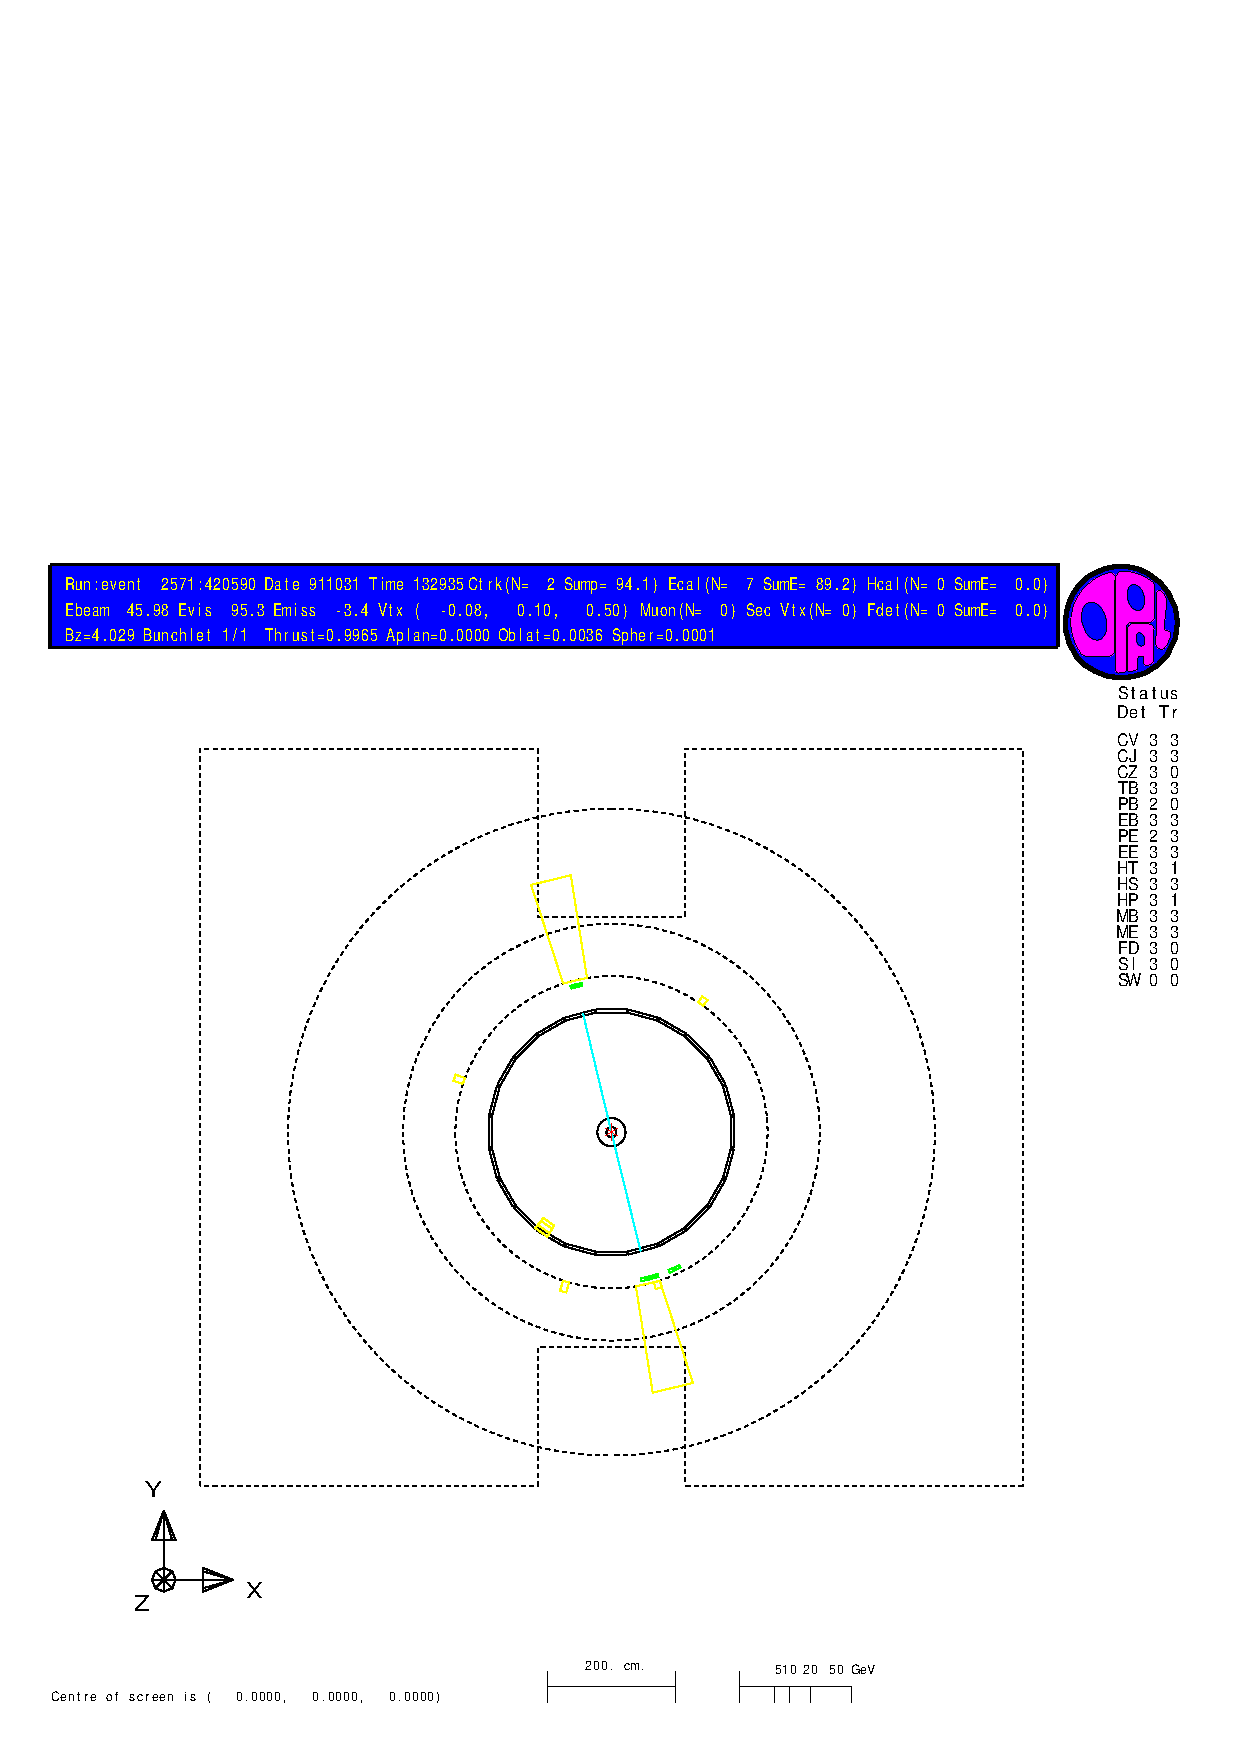
\includegraphics[width=\linewidth]{opal-electrons}
        \caption{%
            Electrons
        }
        \label{fig:grope/electrons}
    \end{subfigure}
    \hfill
    \begin{subfigure}[c]{0.48\linewidth}
        \centering
        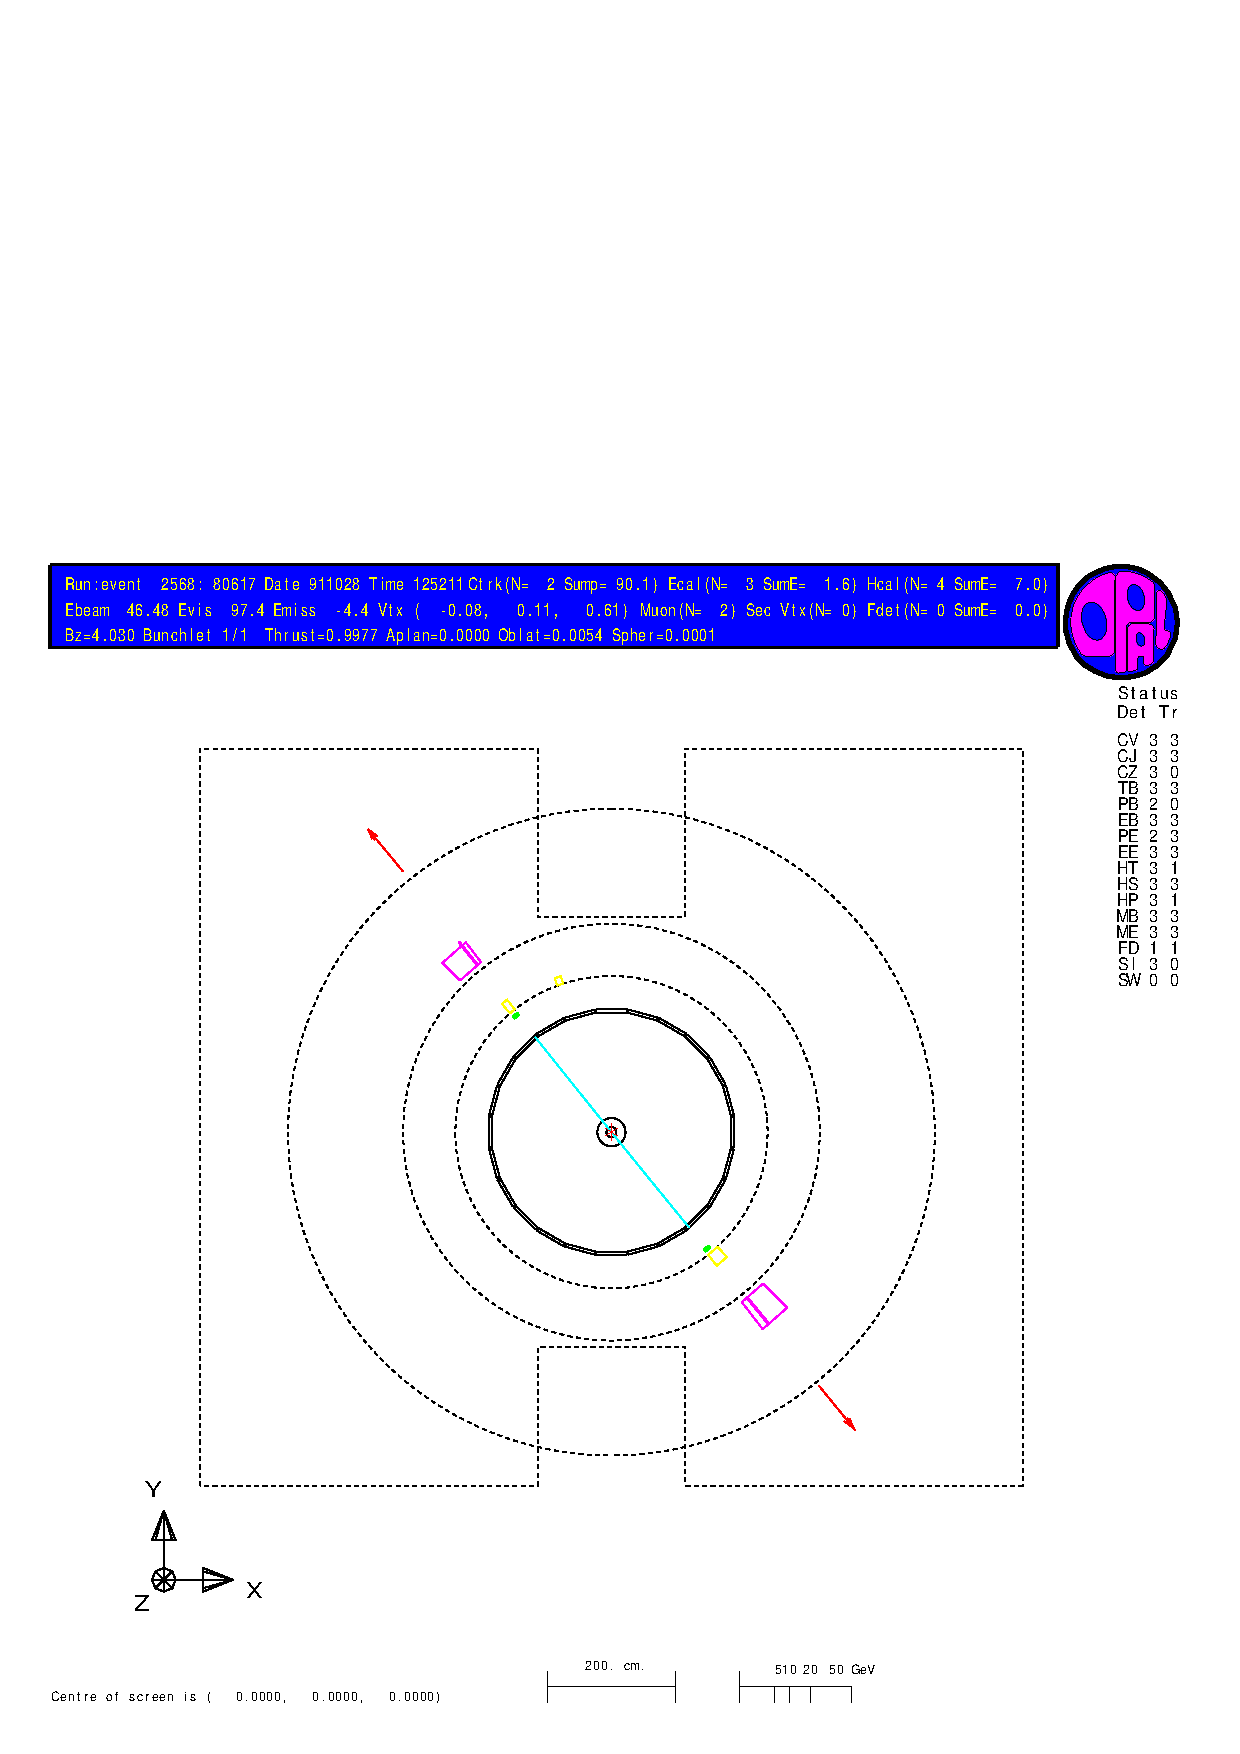
\includegraphics[width=\linewidth]{opal-muons}
        \caption{%
            Muons
        }
        \label{fig:grope/muons}
    \end{subfigure}

    \vspace{2ex}

    \begin{subfigure}[c]{0.48\linewidth}
        \centering
        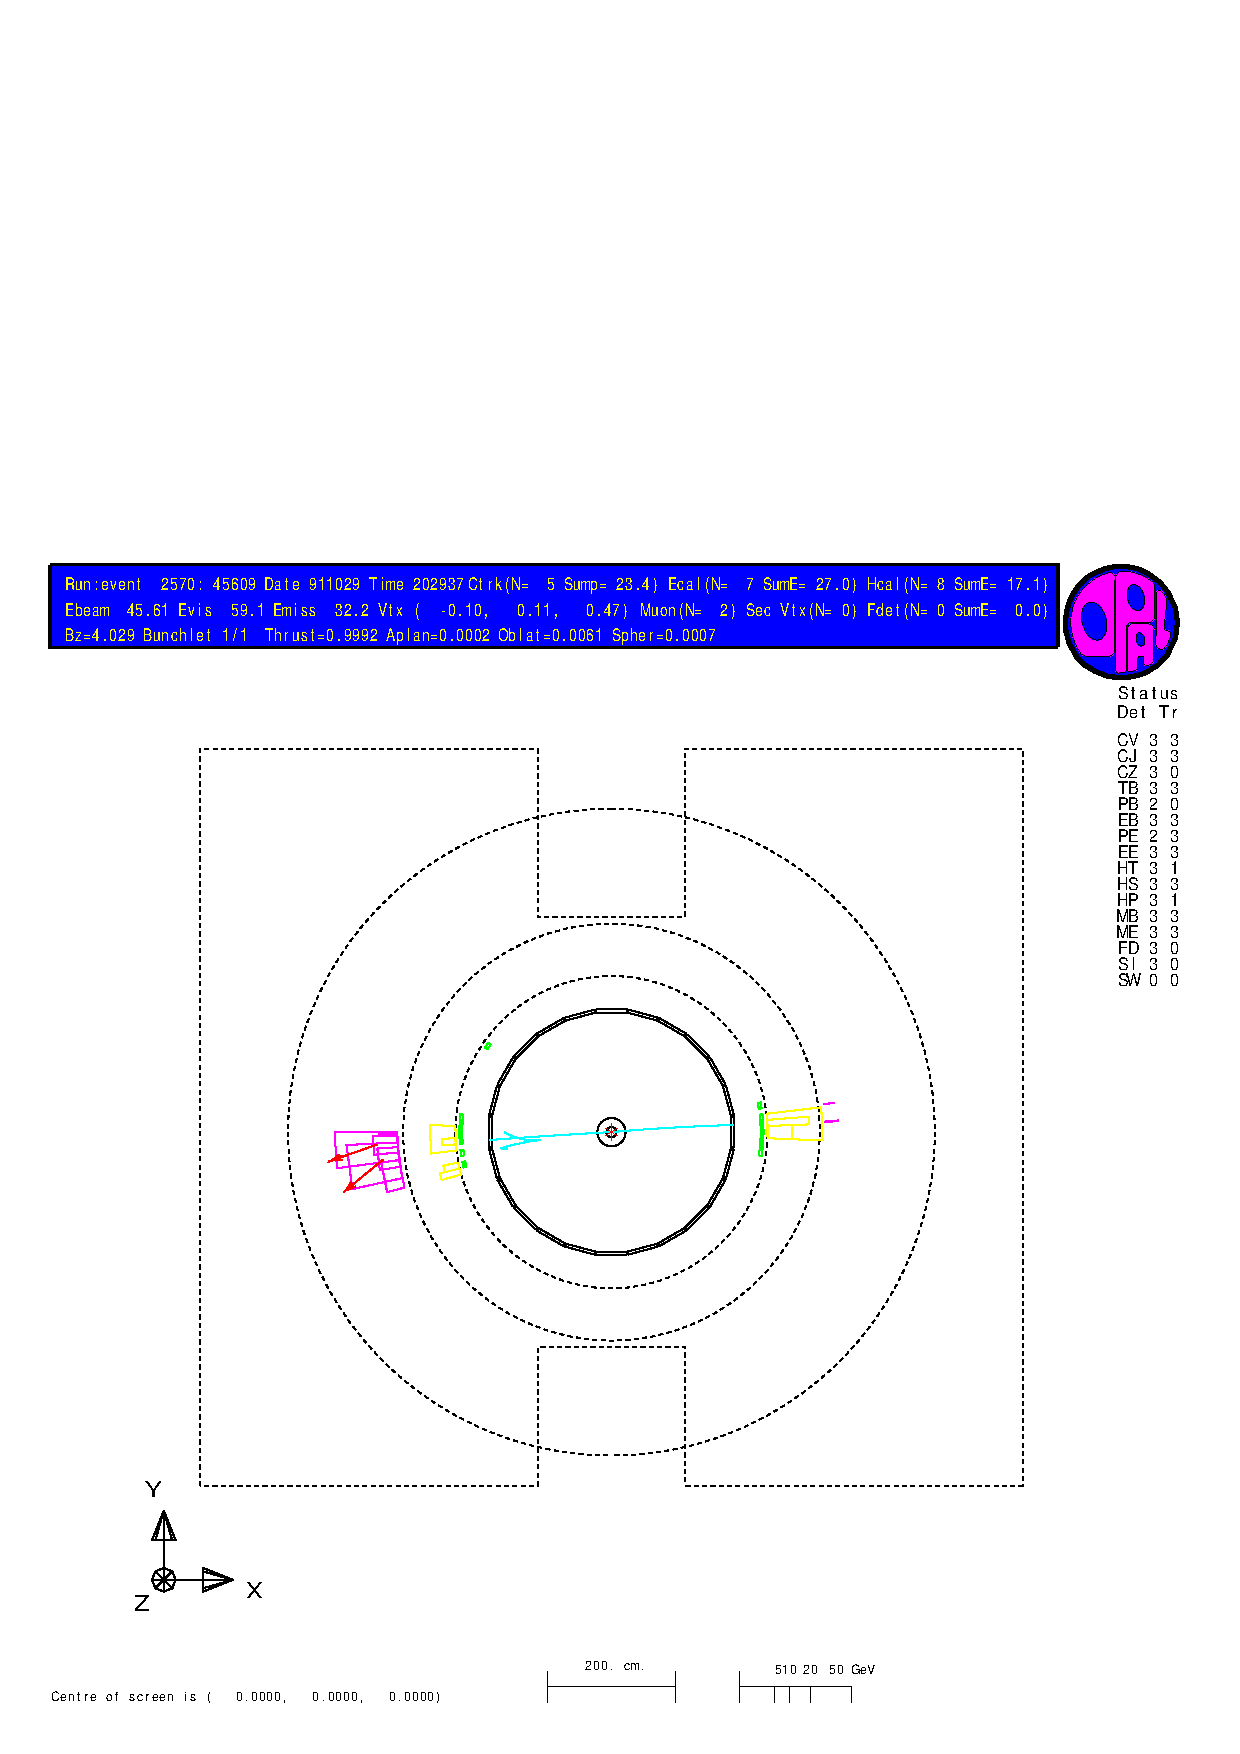
\includegraphics[width=\linewidth]{opal-taus}
        \caption{%
            Taus
        }
        \label{fig:grope/taus}
    \end{subfigure}
    \hfill
    \begin{subfigure}[c]{0.48\linewidth}
        \centering
        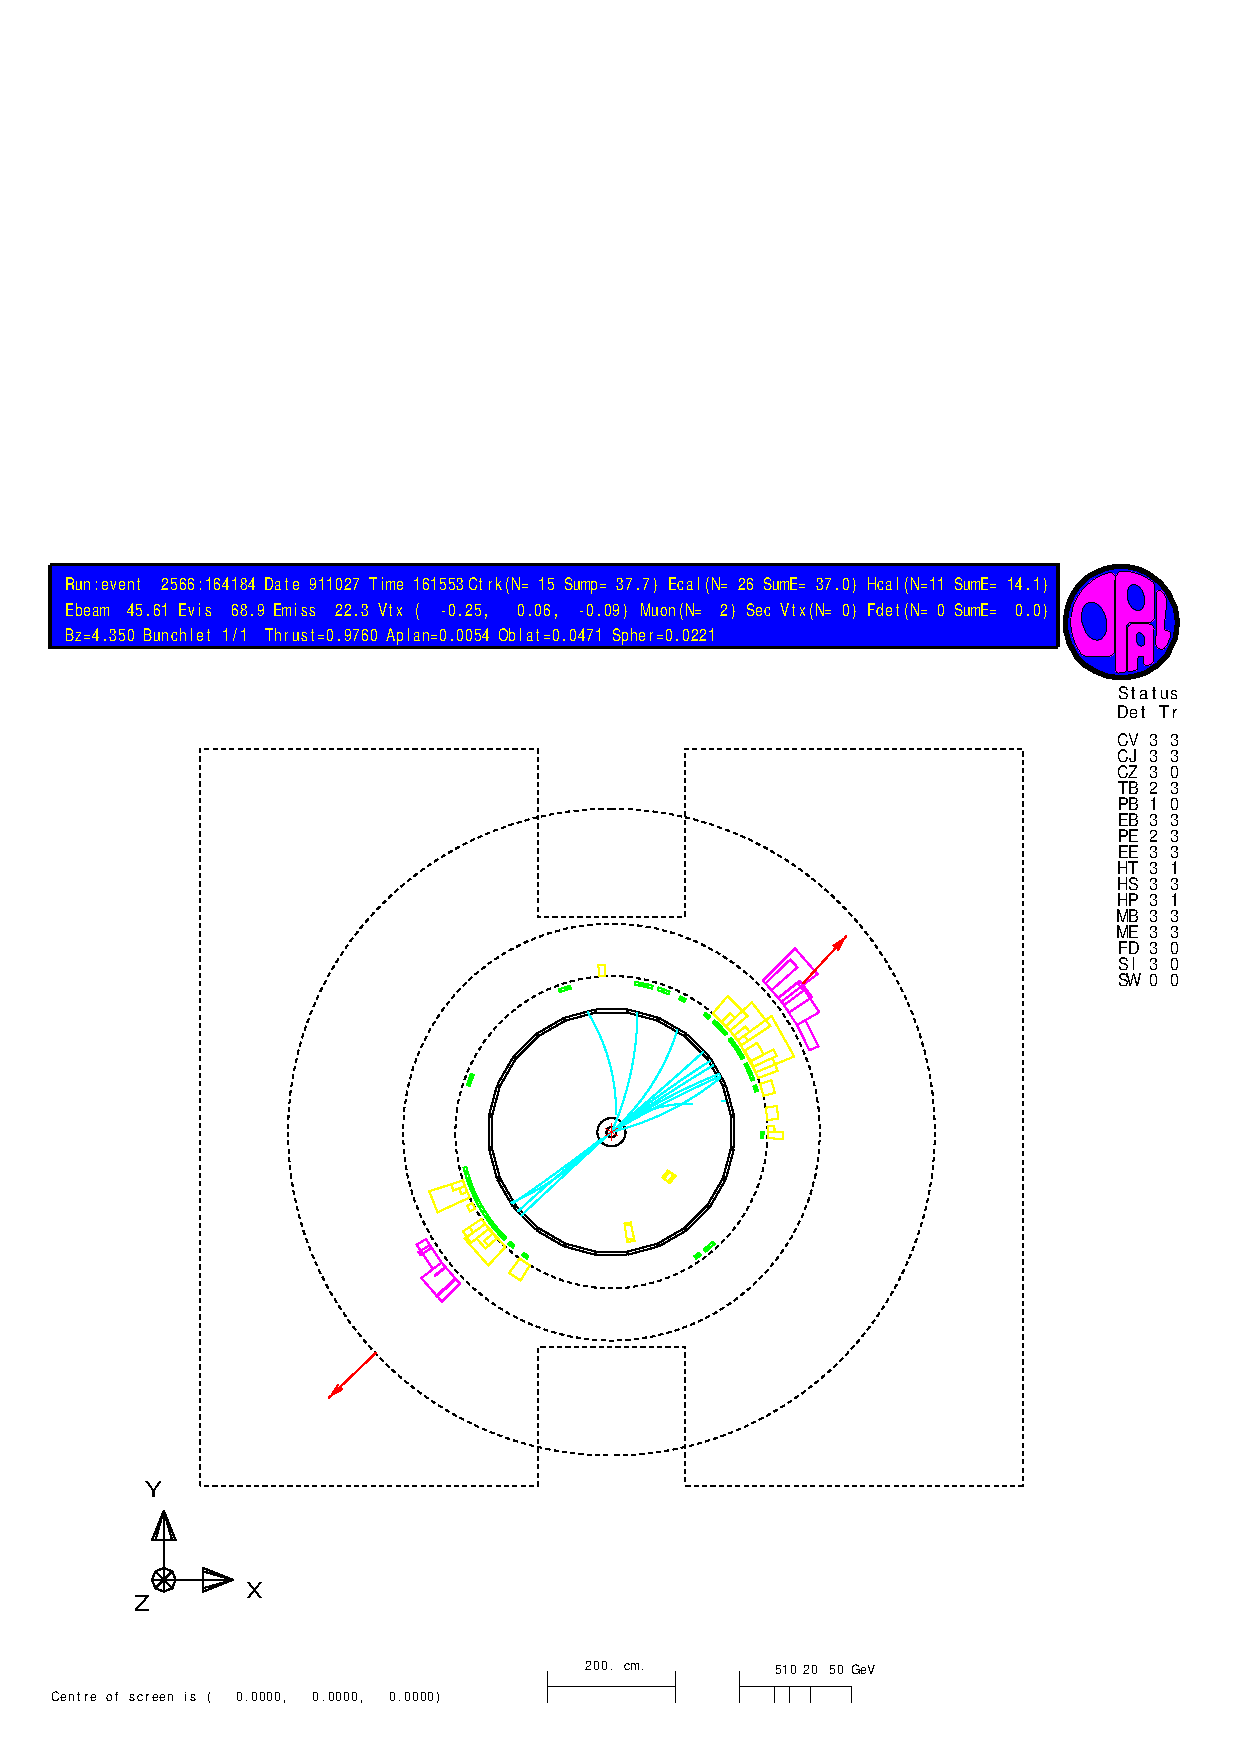
\includegraphics[width=\linewidth]{opal-hadrons}
        \caption{%
            Hadrons
        }
        \label{fig:grope/hadrons}
    \end{subfigure}
    \caption{%
        Event display of Monte Carlo events. One can see the traces from the
        vertex chamber in cyan, the hits in the \ecal{} are shown in yellow
        (probably hard to see on paper). In magenta, one has the hits in the
        \hcal{}. Muon penetrations are indicated with red arrows. Images are
        rendered with \textsc{grope}.
    }
    \label{fig:grope}
\end{figure}

The electron decay in Figure~\ref{fig:grope/electrons} shows the typical
back-to-back signature of two very fast (no curvature in the vertex chamber)
charged particles. All the energy is deposited in the \ecal{}. In the dark blue
header one can see that the missing energy is very small. The energy deposited
in the \ecal{} is pretty much identical with \sump{}. Both energies are almost
the beam energy.

Decays into muons have a different signature. The most prominent feature are
the hits in the muon chambers, as one can see in Figure~\ref{fig:grope/muons}.
The \sump{} is the beam energy, little energy is unaccounted for. This means
that there are no neutrinos created in that decay. The energies deposited in
\ecal{} and \hcal{} is small, this is due to the big mass of the muon (compared
to electrons).

Figure~\ref{fig:grope/taus} shows a decay into taus. This decay is not as
simple as the previous ones. We have some missing energy (around a third), more
than one charged track and also energy deposited into the various calorimeters.
The missing energy comes from the neutrinos in the weak decay of the tau. The
number of charged tracks is still small (just five), therefore we can
differentiate from the hadronic decays.

Lastly, a decay into hadrons is shown in Figure~\ref{fig:grope/hadrons}. One
directly sees the large number of tracks (26) which exhibit a larger curvature.
Also we have energy deposited into \hcal{}. Hadronic decays are easy to
classify as their number of charged tracks is always rather large.

\section{Defining the cuts}

\begin{figure}
    \centering
    \includegraphics[width=\linewidth]{mpl-hist}
    \caption{%
        Histograms with data gathered from Monte Carlo datasets in
        \textsc{grope}. The number of charged tracks is shown as a histogram
        with logarithmic bins.
    }
    \label{fig:mpl-hist}
\end{figure}

\begin{figure}
    \centering
    \includegraphics[width=\linewidth]{mpl-scatter}
    \caption{%
        3D visualization of the three best characteristics.
    }
    \label{fig:mpl-scatter}
\end{figure}

\begin{figure}
    \centering
    \begin{subfigure}[t]{0.48\linewidth}
        \centering
        \includegraphics[width=\linewidth]{mpl-normalized_matrix}
        \caption{%
            Detection matrix. Left-multiply with a vector which contains actual
            event numbers to get event numbers identified by our cuts.
        }
        \label{fig:/1}
    \end{subfigure}
    \hfill
    \begin{subfigure}[t]{0.48\linewidth}
        \centering
        \includegraphics[width=\linewidth]{mpl-inverted_matrix}
        \caption{%
            Inverse matrix. Left-multiply with a vector containing our
            measurements to get actual event numbers.
        }
        \label{fig:/2}
    \end{subfigure}
    \caption{%
        Normalized conversion matrices between detected and actual event types.
    }
    \label{fig:}
\end{figure}

\section{Muon forward--backward asymmetry}

\begin{figure}
    \centering
    \includegraphics{plot-afb}
    \caption{%
        Forward--backward asymmetry in the muon events. Shown are both
        uncorrected and corrected values for $A_\text{FB}$. Both values have
        the same error, therefore we only show the error bar for the corrected
        values.
    }
    \label{fig:plot-afb}
\end{figure}

\section{Partial cross sections}

\begin{figure}
    \centering
    \includegraphics{cross-sections}
    \caption{%
        Partial cross sections for each type of final state. One can see that
        the leptonic cross sections are all similar, as expected. The hadronic
        cross section has to be $N_\text f N_\text c = 5 \cdot 3 = 15$ larger
        than the one in the single leptonic channels.
    }
    \label{fig:cross-sections}
\end{figure}

\section{Decay widths}


\end{document}

% vim: spell spelllang=en_us tw=79
